% !TEX program = lualatex
% Unofficial University of Cambridge Poster Template
% https://github.com/andiac/gemini-cam
% a fork of https://github.com/anishathalye/gemini
% also refer to https://github.com/k4rtik/uchicago-poster

\documentclass[final]{beamer}

% ====================
% Packages
% ====================

\usepackage[T1]{fontenc}
\usepackage{lmodern}
\usepackage[orientation=portrait,size=a2,scale=1.15]{beamerposter}
\usetheme{gemini}
\usecolortheme{nott}
\usepackage{graphicx}
\usepackage{booktabs}
\usepackage{tikz}
\usepackage{pgfplots}
\pgfplotsset{compat=1.14}
\usepackage{anyfontsize}
\usepackage{enumerate}
\usepackage{mathtools}
\usepackage{subcaption}
\usepackage{bm}


\usepackage{amsmath,amssymb}

\newcommand{\R}{\mathbb{R}}
\newcommand{\bsi}{{\bf a}}
\newcommand{\E}{\mathcal{E}}
\newcommand{\N}{\mathbb{N}}
\newcommand{\T}{\mathcal{T}}
\newcommand{\F}{\mathcal{F}}
\newcommand{\Kx}{\mathcal{K}}
\newcommand{\K}{\mathcal{K}_{\text{vor}}}
\newcommand{\M}{\mathscr{M}}
\newcommand{\A}{\textbf{a}}
\newcommand{\Ka}{\mathcal{K}_A}
\newcommand{\I}{\mathcal{I}}
\newcommand{\si}{a}
\newcommand{\xkjtrial}{x^{k,j}_{\mathrm{trial}}}
\newcommand{\flow}{f_{\mathrm{low}}}
\newcommand{\simplex}{\textstyle\sum}
\DeclareMathOperator*{\Div}{div}
\DeclareMathOperator*{\rank}{rank}
\DeclareMathOperator*{\inter}{int}
\newcommand{\mL}{\mathcal{K}_{\textrm{vor}}}

\newcommand{\mV}{\bm{V}}


% ====================
% Lengths
% ====================

% If you have N columns, choose \sepwidth and \colwidth such that
% (N+1)*\sepwidth + N*\colwidth = \paperwidth
\newlength{\sepwidth}
\newlength{\colwidth}
\setlength{\sepwidth}{0.025\paperwidth}
\setlength{\colwidth}{0.45\paperwidth}

\newcommand{\separatorcolumn}{\begin{column}{\sepwidth}\end{column}}

% ====================
% Title
% ====================

\title{\LARGE Título del trabajo}

\author{\large Autor 1 \inst{1} \and Autor 2 \inst{1} \and Autor 3 \inst{2}}

\institute[shortinst]{\inst{1} Universidad 1 \samelineand \inst{2} Universidad 2}

% ====================
% Footer (optional)
% ====================

\footercontent{
  EIMAT 2026\hfill
  \href{mailto:gdquintero@mail.uniatlantico.edu.co}{gdquintero@mail.uniatlantico.edu.co}}
% (can be left out to remove footer)


% use this to include logos on the left and/or right side of the header:
\logoright{\begin{minipage}{10cm}

\includegraphics[height=4.5cm]{logo_eimat_blanco.png} 
\end{minipage}}
\logoleft{\hspace{20ex}
\includegraphics[width=3cm]{logo_ua_vertical_blanco.png}}

% =========================
% AQUI EMPIEZA EL DOCUMENTO
% =========================

\begin{document}
\begin{frame}[t]

% PRIMERA COLUMNA DEL PÓSTER
\begin{columns}[t]
\separatorcolumn
\begin{column}{\colwidth}

\begin{block}{Resumen}
En este trabajo, investigamos la optimización de Teselaciones de Voronoi Centroidales (CVT) bajo restricciones geométricas. Con este propósito, minimizamos una combinación lineal del funcional de energía estándar de CVT con términos que involucran atributos geométricos, como área y perímetro. La derivada del funcional objetivo con respecto a la posición de los generadores se calcula utilizando técnicas de cálculo de formas y análisis de sensibilidad de diagramas de minimización. Se presentan diversos experimentos numéricos para explorar restricciones geométricas, tales como celdas con áreas idénticas, celdas sin aristas pequeñas y distribuciones de celdas basadas en densidad.
\end{block}

\begin{block}{Diagrama de Voronoi}
Sea $P\coloneq\lbrace a_i \rbrace_{i\in\K}$ un conjunto de puntos dados con $a_i\neq a_j$ para $i\neq j$ e $i,j\in \K\coloneq\lbrace 1, \cdots, \kappa_0 \rbrace$ donde $2\leq\kappa_0 < \infty$. La $i$-ésima celda de Voronoi está dada por
\begin{equation}
\small V_i := \lbrace x\in \R^2|\quad \|x-a_i\| \leq \| x-a_j \| \text{ para } i\neq j \text{ y } j\in \K  \rbrace,
\end{equation}
y el conjunto $\mV(\bsi)=\{V_i(a_i)\}_{i\in \K}$ es el diagrama de Voronoi generado por $P$
\end{block}

\begin{exampleblock}{Análisis de sensibilidad de diagramas de Voronoi}
    \begin{enumerate}
        \item El objetivo general es calcular la derivada de funciones $\bsi\mapsto G(\bsi)$ que dependen de la forma del diagrama de Voronoi $\mV(\bsi)$.
        \item Se introduce una perturbación de los sitios $\bsi+t\delta\bsi$, donde $\delta\bsi := \{\delta a_k\}_{k\in\mL}$ es una dirección de perturbación prescrita, y $t\in \R$ es un parámetro escalar pequeño.
        \item La derivada direccional de $G$ en la dirección $\delta \bsi$ es
        $$ \small\nabla G(\bsi) \cdot \delta\bsi = \lim_{t\to 0} \frac{G(\bsi+t\delta\bsi) - G(\bsi)}{t}.$$
        \item Nuestro algoritmo numérico está basado en el gradiente $\nabla G(\bsi)$.
        \item La perturbación de los sitios induce un diagrama de Voronoi perturbado, denotado por 
        $\mV(\bsi+t\delta\bsi) := \{V_k(\bsi+t\delta\bsi)\}_{k\in\mL}.$
        \item En \cite[\S4]{birgin:01}, se examina un marco teórico para analizar la sensibilidad de diagramas de Voronoi. La idea principal es construir una aplicación $T(\cdot, t)$ que transporta cada celda de referencia $V_k(\bsi)$ hacia su correspondiente perturbada $V_k(\bsi+t\delta\bsi)$.
    \end{enumerate}
    Utilizamos estos resultados en este trabajo.
\end{exampleblock}

\begin{block}{Teselaciones centroidales de Voronoi}
Sea $\rho: A\to \R$, $\rho >0$, una función de densidad dada.
El centroide de masa de una celda de Voronoi $V_i(\bsi)$ se define por
$$
\small c_i := \frac{\displaystyle \int_{V_i(\bsi)} x \,\rho(x)\,dx}{\displaystyle \int_{V_i(\bsi)} \rho(x)\,dx}.
$$
En general, tenemos $c_i \neq \si_i$. Cuando $c_i= \si_i$ para todo $i=1,\dots,\kappa_0$, $\mV(\bsi)$ se denomina Teselación de Voronoi Centroidal (CVT)
\end{block}
\begin{block}{Construcción de CVTs}
Consideramos el siguiente problema de optimización
\begin{equation*}
\small\min_{\bsi\in \R^{2\kappa_0}} G(\bsi)
\end{equation*}
considerando el dominio $A=[0,\sqrt{\kappa_0}]$, donde $\small G(\bsi)\coloneq \frac{1}{\kappa_0}\sum^{\kappa_0}_{i=1} G_i(\bsi) \text{ con } G_i(\bsi) = \displaystyle\int_{V_i(\bsi)}\|x-a_i\|^2\,dx$ es la función de energía de CVT. Utilizando técnicas de cálculo de formas y los resultados presentados en \cite{birgin:01}, calculamos dos expresiones para el gradiente de $G(\bsi)$.
\end{block}

\begin{alertblock}{Dos expresiones para el gradiente de $G(\bsi)$}
La primera consiste en considerar la forma integral de $G(\bsi)$
\begin{equation}
    \footnotesize \nabla G(\bsi)\cdot \delta \bsi = \frac{1}{\kappa_0}\sum^{\kappa_0}_{i=1} 2 \delta a_i \cdot (a_i - c_i)|V_i(\bsi)|. \label{grad1}
\end{equation} 
La segunda forma es calcular explícitamente el valor de $G(\bsi)$, realizando un cambio de variables; entonces, el gradiente está dado por
\begin{equation}\label{grad2}
\footnotesize \nabla G(\bsi) \cdot \delta \bsi = \frac{1}{\kappa_0}\sum^{\kappa_0}_{i=1}\nabla G_i(\bsi)\cdot \delta \bsi,
\end{equation}
con
\begin{align}
\footnotesize\begin{split}
     \nabla G_i(\bsi)\cdot \delta \bsi &= \frac{1}{12}\sum_{E\in \E_i}\F(i,v_E)\cdot(\kappa_i(E)(-w^\perp_E + a^\perp_i) + |\det D\phi|(2v_E+w_E-3a_i)) \\
    & +\F(i,w_E)(\kappa_i(E)(v^\perp_E-a^\perp_i)+|\det D\phi|(v_E+2w_E-3a_i)\\
    &-\delta a_i \cdot (\kappa_i(E)(-w_E^\perp+v^\perp_E)+3|\det D\phi|(v_E+w_E-2a_i) )\end{split}, \label{grad2}
\end{align}
donde 
\begin{equation*}
    \footnotesize \kappa_i(E)=\text{sign}(\det D\phi)(\|v_E-a_i\|^2+(v_E-a_i)\cdot(w_E-a_i)+\|w_E-a_i\|^2).
\end{equation*}
\end{alertblock}
\end{column}

% SEGUNDA COLUMNA DEL PÓSTER
\separatorcolumn

\begin{column}{\colwidth}
\begin{block}{Construcción de teselaciones de Voronoi centroidales con propiedades específicas}
\begin{enumerate}
    \item \textbf{CVTs con celdas de volumen idéntico.}
    Consideramos la función de mérito dada por
{\small\begin{equation*}
    f_1(\bsi):= \omega G(\bsi) + J^1(\bsi),
\end{equation*}}
donde,
{\small\begin{equation*}
    J^1(\bsi) := \frac{1}{\kappa_0}\sum^{\kappa_0}_{i=1}[J^1_i(\bsi)]^2, \text{ con }     J^1_i(\bsi):=\left(\int_{V_i(\bsi)}\,dx\right)/\left(\frac{1}{\kappa_0}\int_A \, dx \right)-1,
\end{equation*}}
\begin{figure}[ht!]
\begin{subfigure}{0.28\linewidth}
\centering
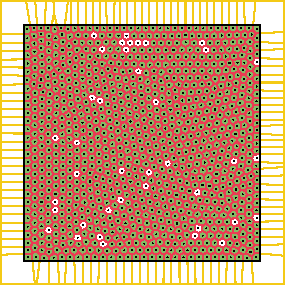
\includegraphics[scale=0.75]{imagenes/bfl2024fig24.pdf}
\caption{Min $G(\bsi)$}
\label{fig:j3a}
\end{subfigure}
\begin{subfigure}{0.28\linewidth}
\centering
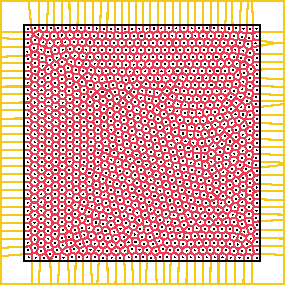
\includegraphics[scale=0.75]{imagenes/bfl2024fig25.pdf}
\caption{Min $f_1(\bsi)$ con $\omega=0.001$} 
\label{fig:j3b}
\end{subfigure}
\caption{Teselación de Voronoi centroidal con $\kappa_0=1000$ buscando celdas de área idéntica.}
\end{figure}
\item \textbf{CVTs con restricciones en la longitud de las aristas.} Consideremos ahora la siguiente función objetivo
{\small\begin{equation*}
    f_2(\bsi) \coloneq \omega G(\bsi) + J^2(\bsi),
\end{equation*}}
donde 
{\small\begin{align*}
    J^2(\bsi) \coloneq\sum^{\kappa_0}_{i=1}J^2_i(\bsi) \text{ con } J^2_i(\bsi) := \frac{1}{n_i}\sum_{E\in \E_i}\min\left\lbrace 0, \frac{|E|}{\bar{E}_i}-c_2 \right \rbrace^2 \label{eq:J1}.
\end{align*}}
\begin{figure}[ht!]
\begin{subfigure}{0.2 \linewidth}
\centering
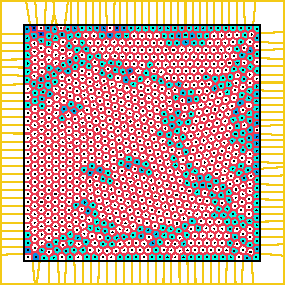
\includegraphics[width=\linewidth]{imagenes/bfl2024fig7a.pdf}
\caption{$G(\bsi)$ \\ \quad}
\end{subfigure}
\begin{subfigure}{0.2 \linewidth}
\centering
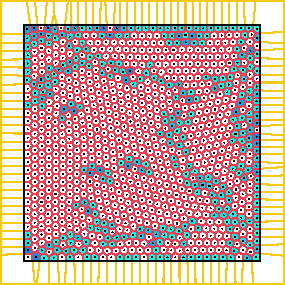
\includegraphics[width=\linewidth]{imagenes/bfl2024fig7b.pdf}
\caption{$f_2(\bsi)$ con $c_2=0.3$} 
\end{subfigure}
\begin{subfigure}{0.2 \linewidth}
\centering
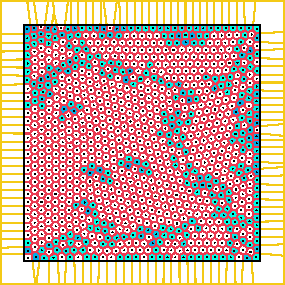
\includegraphics[width=\linewidth]{imagenes/bfl2024fig7c.pdf}
\caption{$f_2(\bsi)$ con $c_2=0.4$}
\end{subfigure}
\begin{subfigure}{0.2 \linewidth}
\centering
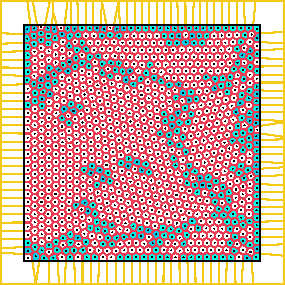
\includegraphics[width=\linewidth]{imagenes/bfl2024fig7d.pdf}
\caption{$f_2(\bsi)$ con $c_2=0.5$} 
\end{subfigure}
\begin{subfigure}{0.2 \linewidth}
\centering
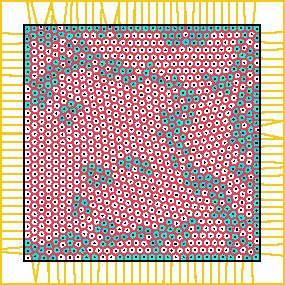
\includegraphics[width=\linewidth]{imagenes/bfl2024fig7e.pdf}
\caption{$f_2(\bsi)$ con $c_2=0.6$}
\end{subfigure}
\begin{subfigure}{0.2 \linewidth}
\centering
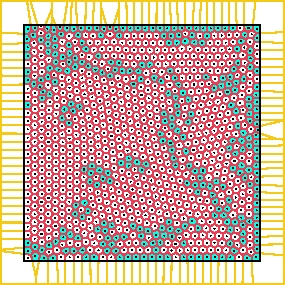
\includegraphics[width=\linewidth]{imagenes/bfl2024fig7f.pdf}
\caption{$f_2(\bsi)$ con $c_2=0.7$} 
\end{subfigure}
\begin{subfigure}{0.2 \linewidth}
\centering
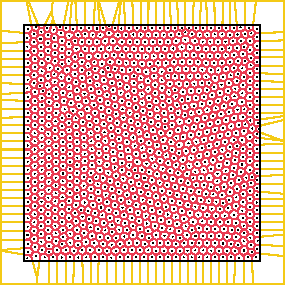
\includegraphics[width=\linewidth]{imagenes/bfl2024fig7g.pdf}
\caption{$f_2(\bsi)$ con $c_2=0.8$}
\end{subfigure}
\captionsetup{list=no}
\caption{Teselaciones de Voronoi centroidales con $\kappa_0=1000$ evitando celdas con aristas pequeñas.}
\label{fig7}
\end{figure}

\item \textbf{Teselaciones de Voronoi centroidales basadas en densidad.} 
\begin{equation*}
    \small f_3(\bsi)=G(\bsi)+J^3(\bsi)
    \label{eq:J3}
\end{equation*}
donde 
\begin{equation*}
    \small J^3(\bsi) := \frac{1}{\kappa_0} \sum^{\kappa_0}_{i=1}[J^3_i(\bsi)]^2 \text{ con } J^3_i(\bsi)\coloneqq \left(\int_{V_i(\bsi)}\,dx\right)/\left(\frac{1}{\kappa_0}\int_A \, dx \right)-\psi(a_i).
\end{equation*}
\begin{figure}[H]
\begin{subfigure}{0.2 \linewidth}
    \centering
    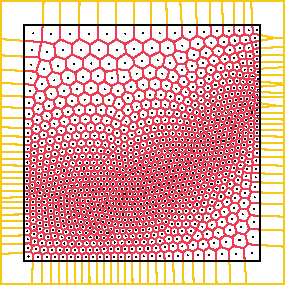
\includegraphics[width=\linewidth]{imagenes/bfl2024fig27.pdf}
    \caption{}
    \label{fig:s2a}
\end{subfigure}
\begin{subfigure}{0.2 \linewidth}
    \centering
    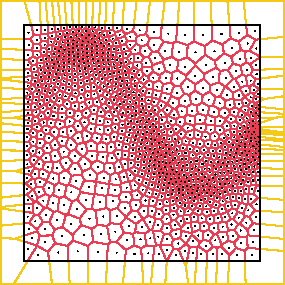
\includegraphics[width=\linewidth]{imagenes/bfl2024fig28.pdf}
    \caption{}
    \label{fig:s2b}
\end{subfigure}
\begin{subfigure}{0.2 \linewidth}
    \centering
    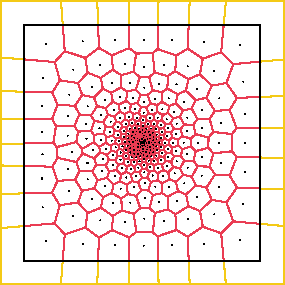
\includegraphics[width=\linewidth]{imagenes/bfl2024fig29.pdf}
    \caption{}
    \label{fig:s4a}
\end{subfigure}
\end{figure}

\begin{enumerate}[a]
\item $\psi(z) = a((\bar{z_2}-(\bar{z_1}/4)^2)^2 + (\bar{z_1}/4-1)^2) + b$, donde $\bar{z} = \frac{2}{5}z-\frac{c}{5}$, con $c$ siendo el centro del cuadrado, $b=0.25$ y $a = \frac{1}{16}(2-b-\frac{9}{16})$.
\item $\psi(z) = 0.1 + \frac{2.9}{\delta^2}\left(z_2-0.6\delta \sin(\frac{2\pi z_1}{\sqrt{\kappa_0}}) - \delta \right)^2$ con $\delta=\frac{\sqrt{\kappa_0}}{2}$.
\item $\psi(z)=0.01 + 20\| z-c\|^2/r^2$ donde $c$ y $r$ son el centro y el radio del círculo inscrito en el cuadrado.
\end{enumerate}
\end{enumerate}

\end{block}

  \begin{block}{Referencias}

    \nocite{*}
    \footnotesize{\bibliographystyle{plain}\bibliography{poster}}

  \end{block}

\end{column}
\separatorcolumn

\end{columns}
\end{frame}

\end{document}
